% ============================================================================
%  Chapter 1. Introduction  (Morgan State MS format)
%
%  \input file. No preamble, no font, spacing or margin commands.
%  Parent document supplies: 12pt report class, double spacing, Times,
%  natbib (\citep), booktabs. Bibliography: accord/thesis/refs.bib
%
%  Every number in this chapter is keyed to results/accord/VERIFIED_FACTS.json.
%  Nothing is carried over from an earlier draft without a key.
%
%  The control-literature attributions are now wired to refs.bib: Lipsitch,
%  Adebayo, Hewitt & Liang, Egami, Forman, Feinstein, Byrt, Lourie, TESSERA,
%  Pfohl, Fogliato, Biswas & Rajan, Jacobs and DeLong.
%
%  Figures: fig:pipeline-status (Section "The Pipeline the Field Would Build")
%  and fig:intro-headline (Section "The Finding"). Both are rendered by
%  accord/thesis/figures/make_figures.py from committed result files; see
%  figures/manifest.json for the per-panel source list.
% ============================================================================

\chapter{Introduction}
\label{ch:intro}

\section{A Patient Goes Home on a Medication That Was Held}
\label{sec:intro-problem}

A patient admitted for decompensated heart failure spends nine days on the
service. On day four a nurse writes that the loop diuretic was held because the
patient had become hypovolemic. On day nine the discharge summary lists that
same diuretic among the medications to continue at the admission dose. Both
documents are in the chart, both record what someone believed when they wrote
it, and they disagree.

The disagreement matters because the two documents do not have equal reach. The
discharge summary is what the outpatient physician reads, what the pharmacy
fills against, and what the patient's family is handed. The nursing note holding
the reason the instruction is wrong is unlikely to travel with the patient. A
contradiction of this kind is not a documentation defect that gets cleaned up
later. It is an instruction that leaves the building.

The scenario above is a constructed composite, drawn from no single record in
this project's corpus; the pattern it illustrates is real. Of the $12$
contradictions a board-certified pharmacist confirmed in this project's
annotated sample, $3$ involve a loop
diuretic and $3$ involve an anticoagulant, $7$ have a clinical failure mode the
pharmacist coded as omission rather than as a dose or class disagreement, and
on a five point danger scale $1$ was rated $4$ and $3$
were rated $5$. The category is small, and the members of it are the drugs where
a wrong instruction does damage quickly.

None of this is rare at the level of the health system. Unintended medication
discrepancies are present in a large share of admissions
\citep{cornish2005discrepancies} and of discharges
\citep{wong2008reconciliation}. Adverse events in the weeks after discharge are
common, frequently drug related, and frequently preventable
\citep{forster2003adverse}. Errors traceable to discontinuity between inpatient
and outpatient care affect a substantial fraction of discharged patients
\citep{moore2003discontinuity}, and the information transfer that would prevent
them is unreliable in both content and timing \citep{kripalani2007deficits}.
Adverse drug events were established as a first order inpatient safety problem
three decades ago \citep{bates1995ade}, and the transition of care component of
that problem has not been solved since.

This thesis takes one narrow, checkable instance as its object. A
\emph{cross-note medication contradiction} is a disagreement about a specific
drug between a nursing progress note and the discharge summary of the same
admission. The
corpus is MIMIC-III \citep{johnson2016mimic}, accessed under PhysioNet
credentialed use. No note text and no identifiers appear anywhere in this
document, and every quantity reported is an aggregate.

The phenomenon is real and it is rare. The pharmacist annotated $299$ candidate
pairs and confirmed $12$, a base rate of $0.0401$ in a pool four hand written
rules had already enriched. Restricting to the $253$ pairs the annotator did not
mark ambiguous leaves the same $12$ positives, a base rate of $0.0474$. Those
two denominators, $299$ and $253$, are different sets. They are kept apart
everywhere in this thesis, because an earlier draft conflated them and inverted
a central claim in the process. Rarity is not a nuisance parameter here. It is
what breaks every stage of the pipeline described next.

\section{The Pipeline the Field Would Build}
\label{sec:intro-pipeline}

Given a rare event, expensive expert labels, and a large corpus of paired notes,
the standard construction is close to automatic. Mine candidates with cheap high
recall rules, because exhaustive expert review of every cross-note medication
pair is infeasible. Label those candidates with an instruction tuned language
model, because expert annotation does not scale and recent work reports such
models matching or exceeding crowd annotators on several classification tasks
\citep{gilardi2023chatgpt}. Distil the labels into a purpose-built neural
detector, referred to throughout this thesis as ACCORD, over a domain-pretrained
clinical encoder
\citep{gu2021biomedbert,alsentzer2019clinicalbert}, with architectural
components that encode the structure a generic natural language inference model
lacks. Evaluate against the expert annotations and report.

Each step has a literature behind it. Programmatic weak supervision is a mature
line of work with a body of positive results
\citep{ratner2016dataprogramming,ratner2017snorkel}, encoder models classify
entailment between clinician authored sentence pairs at usable accuracy
\citep{romanov2018mednli}, and domain pretraining is the default starting point
for clinical text \citep{gu2021biomedbert}. The construction is defensible at
every step, and this project executed it end to end.

What the construction does not come with is a control at each stage. A candidate
miner reports a precision without reporting whether the evidence attached to
each candidate is the evidence that triggered it, which is a question about
whether the quantity measured is the quantity named
\citep{jacobs2021measurement}. A weak labeller reports an agreement rate
without reporting its own marginal against a measured base rate, although
surrogate labels are known to bias what is computed from them even at high
annotator accuracy \citep{egami2023surrogates}, and a classifier whose true
positive and false positive rates differ is a biased prevalence estimator by
construction \citep{forman2008quantifying}. An architectural component reports
an ablation delta without a version of itself that could not possibly work, run
under the same conditions \citep{adebayo2018sanity,hewitt2019control}. An
evaluation reports a null without a positive control establishing that the same
instrument would have resolved an effect if one had been present, which is the
logic negative controls carry in observational research, extended here to the positive direction
\citep{lipsitch2010negative}. Auditing a pipeline stage by stage rather than
end to end is itself an established move, demonstrated for fairness in tabular
preprocessing \citep{biswas2021fairpreprocessing}. Each of these checks is old,
cheap, and owned by someone else. None was run on this pipeline before this
work.

Figure~\ref{fig:pipeline-status} is the whole project in one view: the four
stages that reported a number no standard metric flagged, the check that
catches what each number hid, and the carrier that takes the stage three
defect into every stage after it. The failures sit at
different stages, have different mechanisms, and each has a cheap detector. A project that fixed any one of them
in isolation would still have produced a system with no ranking signal.

Not every verdict in that figure generalises to the same degree, and the
distinction matters because this thesis is candid elsewhere about defects in
its own execution. Three of the verdicts are
properties of the construction itself, not of how carefully this build carried
it out. A pool mined by high-recall rules over a genuinely rare event lands
near a low base rate because that is what high-recall rules do to a rare
event, not because these four rules were written badly. A language-model
labeller asked to flag a rare class at low prevalence over-calls for a reason
that holds for any classifier with imperfect specificity at that prevalence.
That the failure occurs is general; how large it is is not. Three labellers at
the same eight-billion-parameter scale, run on the identical prompt, already
disagree with one another on how large, so magnitude is not even constant
within a single point on a capability axis, and a compliance withdrawal
described in Chapter~\ref{ch:method} removed the only cell this design had
that varied scale; no ordering by capability is established here. An evaluation built
on the number of pharmacist-confirmed positives that exist is limited by that
number regardless of who trains the detector. Those three findings should
generalise in direction to another group that builds a similarly shaped pipeline
on a similarly rare event, and the magnitudes should not be carried across. Four further items do not carry that weight. The reason to take them
seriously is not that they are implementation bugs, a framing that invites
the wrong reading: that this project built a broken system, found it broken,
and is now recommending that people test their code. The reason is where
each failure hid. Three of the four produced a number that passed this
project's own review and would have passed peer review, because no standard
reported metric was sensitive to it, and each has a one-line check that is.
That check, not a general call for more testing, is the transferable
finding.

The first is a bug class this thesis names \textbf{trigger-exemplar
dissociation}: a mining rule whose predicate quantifies over a set of
candidate mentions, an exemplar selector that picks from that set by
position rather than by membership, and no assertion anywhere tying the two
together. The form generalises to any pipeline built the same way; the check
is one line, asserting that the selected exemplar belongs to the set that
satisfied the trigger predicate. Here the exemplar selector indexed
candidates positionally instead of by the evidence the trigger actually used
(Figure~\ref{fig:exemplar}), and the pool's reported precision of $0.0401$
carried no trace of it, because no metric computed on the pool compares the
displayed evidence against the triggering evidence.

\begin{figure}[!ht]

\centering
\caption[Schematic of the exemplar defect]{The check that was not run. The rule
fires on a conflict between two sets of medication mentions; the exemplar shown
to annotator, weak labeller and model is chosen by position instead. Slots are
abstract and carry no clinical text.}
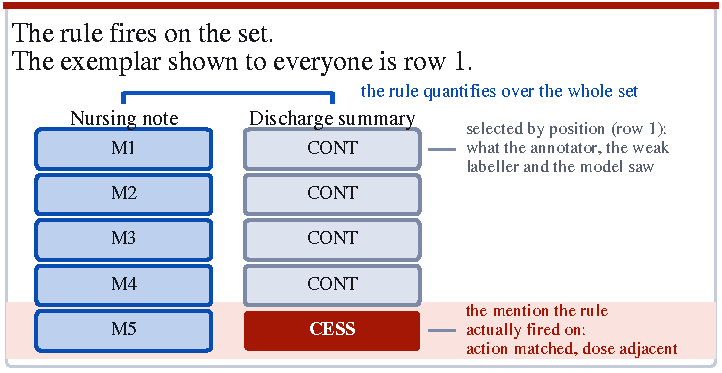
\includegraphics[width=0.88\linewidth]{figures/fig-exemplar.pdf}
\label{fig:exemplar}
\end{figure}

The second is the harm
head, which received no term in the training objective, so its reported
outputs are an untrained module's, invisible to an ablation delta and caught
only by checking a parameter's displacement from its own initialisation
(Chapter~\ref{ch:method}). The third is the row-level candidate split,
corrected to subject-level before any result in this document was generated
(Chapter~\ref{ch:method}): it contaminates whatever metric is computed
downstream of it without moving that metric's own diagnostics, and the check
is a subject-disjointness assertion between the two splits. The fourth,
scispaCy and medspaCy abandoned over dependency resolution rather than
evaluated and rejected, is a scope limitation rather than a metric-blind
defect: no reported number in this thesis depends on that choice, and no
check applies to it.

The multiplier that stage four carries is the weak labeller's positive rate on
the $299$-pair gold set over the pharmacist's base rate on those same $299$
pairs. Both terms are counted on the same rows.

\begin{figure}[!t]

\caption[The pipeline stage by stage]{The four stages whose reported number no
standard metric flagged, each with the check sensitive to what it hid. Stages
$1$ and $2$ reconcile in count and were never diagnosed. The scarlet carrier
marks the stage $3$ exemplar defect, which the weak labeller, the detector and
the pharmacist each saw; it records shared input, not cause. The architecture
row is categorical because no committed result file carries a number for it.}
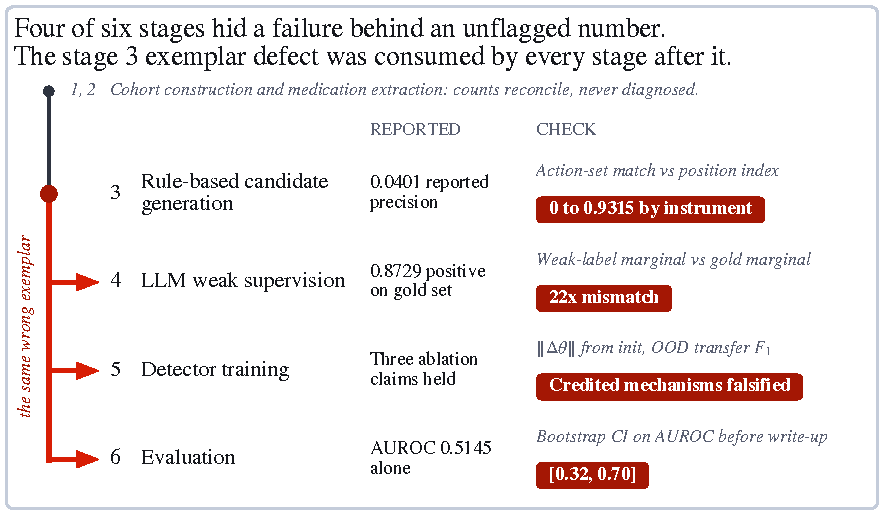
\includegraphics[width=0.98\linewidth]{figures/fig-pipeline-status.pdf}
\label{fig:pipeline-status}
\end{figure}

\section{The Finding}
\label{sec:intro-finding}

The pipeline does not work. This thesis establishes where it fails and why, by
running at each stage the control that separates a real result from an
artifact of the measurement; every stage failed its control, a statement made
once here so nothing later reads as a reveal. The cleanest single expression
of the failure is the decontaminated detector's operating behaviour on the
$253$ non-ambiguous pairs: at the configured threshold it predicts positive
for nearly the whole pool rather than ranking within it, and its ranking is at
chance rather than merely inaccurate, with Cohen's $\kappa$, the calibration
error, and the ensemble AUROC and its bootstrap interval reported at full
precision in Chapter~\ref{ch:results} (Section~\ref{sec:res-rq4},
Table~\ref{tab:decontam}) rather than restated here. Figure~\ref{fig:ceiling}
in Chapter~\ref{ch:results} carries the mechanism behind it: the largest
agreement any thresholded labeller could reach at the weak labeller's positive
rate on the $299$-pair gold set, against the pharmacist's base rate on those
same pairs, which is the marginal RQ2 below reports and RQ4 uses as a
precondition rather than an explanation. A TF-IDF
logistic-regression baseline on the $299$ annotated pairs ranks above both
neural configurations this pipeline produced, which is either surface-form
signal or small-sample noise and is not established either way
(Section~\ref{sec:res-rq4}). A null on twelve positives invites one obvious
reading, that the experiment was too small to see anything; the control that
answers it is a positive control run on the identical training and evaluation
harness, on a public benchmark rather than on this pool. Run on AG News under
an adjudication rule committed before the sweep, the resolved pretraining
benefit is $4.53$ accuracy points at convergence; the same harness, applied to
a clinical mortality task built for this control alone, returns a null,
$+0.0031$ (Section~\ref{sec:res-rq4}; Chapter~\ref{ch:discussion},
Section~\ref{sec:disc-null}). What that pairing licenses is that the harness
resolves a real difference at the sample sizes it was given; it says nothing
about the sensitivity of the twelve-positive contradiction evaluation itself,
which is fixed by that evaluation's own class counts and taken up next as a
screening test measured directly on the labellers this pipeline ran, rather
than as a resolution limit alone.


\section{Research Questions}
\label{sec:intro-rqs}

The project was organized around five questions: four about the stages of the
pipeline and one about the field that publishes pipelines like it. Each is
stated as it was posed, followed by the answer in one sentence. Evidence sits in
Chapter~\ref{ch:results}; the control designed for each stage is specified in
Chapter~\ref{ch:method} as a condition set before any result was seen.

\begin{description}

\item[RQ1. Candidate generation.] Can rule-based mining over paired clinical
notes yield a candidate pool with usable precision?
\emph{No: four rules enrich the pool to $12$ true contradictions in $299$
annotated pairs, a base rate of $0.0401$, and the evidence shown for each
candidate was selected independently of the evidence that triggered it, an
instance of the trigger-exemplar dissociation named in
Section~\ref{sec:intro-pipeline}. Section~\ref{sec:intro-contributions} below
gives the measured range at which that defect fired, and
Section~\ref{sec:intro-notclaim} states what it leaves of the $0.0401$
figure.}

\item[RQ2. Weak supervision.] Can a language model weak labeller substitute for
expert annotation at this base rate?
\emph{No: the weak labeller assigned the contradiction class to $261$ of the
$299$ annotated pairs against $12$ true positives, and every labeller tested
over-calls. Three local eight-billion-parameter models, run on an identical
prompt, over-call the candidate pool's confirmed rate by a multiplier from
$15.8196$ to $23.5959$ (Table~\ref{tab:overcalling}); the three already differ
from one another at this single point on any capability axis, and this
design has no compliant second point left to order them by scale. On a
public-text sweep run with the same three models and the same prompt, the
same mechanism tops out at $3.5000$ times (Section~\ref{sec:res-rq2}), so the
direction of the failure transfers across domains and its size does not.
Substitution fails at every local configuration measured; whether it fails
less at a scale this project could not run through a compliant channel is not
established.}

\item[RQ3. Architecture.] Do the proposed architectural components contribute
what they are credited with?
\emph{No, and the controls fire positively rather than by absence of evidence:
the authority parameters reported as learned finish at $0.5076 \pm 0.0006$ and
$1.0038 \pm 0.0010$ against initialisation at $0.5$ and $1.0$, the harm head's
outputs span $0.3977$ to $0.6096$, which is the range of an untrained sigmoid,
and on a second system built for this analysis, a single-seed randomised
control over the same role-label alphabet directionally loses to true role
labels by $0.3277$ nats with no significance claim attached, while an
arbitrary positional ordinal, a different feature rather than a randomised
version of the same one, beats both.}

\item[RQ4. Evaluation.] Can a labeller's capacity to show discrimination
against a gold standard be established before it scores a single pair, from
its marginal alone, and do the labellers this pipeline actually ran fail that
test?
\emph{Yes, and yes. Holding a labeller's flagged count and the gold
standard's confirmed count fixed fixes the best table of agreement that
marginal can ever produce, a ceiling that is arithmetic rather than a
property of what the labeller knows
\citep{feinstein1990paradoxes,cicchetti1990resolving,byrt1993pabak}, applied
here as a precondition rather than an explanation. Measured this way on
eight local labeller-and-basis rows, four could not have rejected the null at
$\alpha = 0.05$ at any outcome their own marginal permitted, because the
smallest one-sided $p$ value their marginal allows already exceeds it, and
four sit exactly on their marginal-implied ceiling, so their reported
agreement reports their flag rate and nothing else. The weak labeller
supplying the detector's training signal, at $261$ of $299$, is one of the
four that could not have rejected the null before it scored a single pair.
This bounds a thresholded decision only: a labeller that emits a continuous
score is not bounded this way, because the operating threshold can be swept,
and a model that flags most of a pool at one threshold can still rank the
pool perfectly at another. Section~\ref{sec:res-rq4} reports the eight rows
in full and states separately what the twelve-positive evaluation's own
class counts fix as a minimum detectable effect, a second and narrower
constraint on the same null.}

\item[RQ5. Practice.] Does published work audit the selection step upstream
of the model it evaluates, the one control this survey was built to measure?
\emph{Rarely, on that one control: on a $75$ paper corpus deliberately
enriched toward work that attends to selection, $4$ papers audit the
selection step under the strict reading and $14$ under the permissive one,
with both readings reported side by side and the gap between them named as a
coding ambiguity rather than resolved in the flattering direction. The survey
speaks to this one adjacent check; it is not evidence about whether published
work runs the other four controls RQ1 through RQ4 applied to this pipeline.}

\end{description}

RQ4 is the load-bearing check, in a stronger sense than a resolution limit
alone would give it. Without it, the weak labeller's marginal reads as one
more number a larger annotation budget might fix. With it, four of the eight
local rows this pipeline measured, including the row that actually supplied
the detector's training signal, could not have cleared the conventional
threshold at any outcome their marginal permitted, which means the ranking
null Section~\ref{sec:res-rq4} reports on the trained detector is not a
surprising failure to explain. It is the outcome the screening test already
predicted before the detector was trained. The twelve-positive evaluation's
own resolution limit, reported separately in Section~\ref{sec:res-rq4}, is a
second and narrower constraint on the same null; the two do not depend on one
another, and neither substitutes for the other.

\section{Contributions}
\label{sec:intro-contributions}

The methods applied in this thesis are not novel and the thesis does not claim
them. Negative controls come from epidemiology, and the positive direction is this thesis's adaptation of them, where that
literature is decades old \citep{lipsitch2010negative}. Randomisation based
sanity checks on learned components come from the saliency map literature
\citep{adebayo2018sanity}. Control tasks for probing classifiers come from work
that owns both the design and its conclusion \citep{hewitt2019control}. The
prevalence dependence of agreement statistics was described thirty-six years ago
\citep{feinstein1990paradoxes,cicchetti1990resolving}, and the adjusted
coefficient proposed in response removes the marginal sensitivity by removing
the marginal information \citep{byrt1993pabak}.
Chapter~\ref{ch:lit} attributes each of these to the work that owns it, and
this chapter's claim is about what they revealed when pointed at this pipeline.

What is new is the measurement on this pipeline and the fact that the controls
were actually run. Seven contributions follow, each stated at the size the
evidence supports, and one further result is reported separately below the
list because it does not meet the bar a contribution should meet. The twelve
confirmed contradictions bound only two of the strands below, the candidate
pool's precision and the detector's ranking nulls; the exemplar audit, the
survey, the convergence sweep, and the mortality control each carry their own
denominator, at the $165$-pair Rule 1 and Rule 2 pool, $75$ papers, $48$
runs, and $6{,}776$ admissions
respectively.

\begin{enumerate}
\item \textbf{Trigger-exemplar dissociation.} A mining rule whose predicate
quantifies over a candidate set while its exemplar selector picks by
position, with no assertion linking the two, silently corrupts the
annotator, the weak labeller, and the detector through the same wrong
exemplar; the one-line fix, asserting the exemplar belongs to the
predicate-satisfying set, would have caught it at no model cost, and on the
$165$-pair Rule 1 and Rule 2 pool it fired at a rate from $0$ to $0.4745$
depending on measurement (Figure~\ref{fig:exemplar},
Chapter~\ref{ch:results}).
\item \textbf{Two cheap, transferable checks: the degeneracy precondition
and sign provenance.} \emph{Degeneracy precondition:} a classifier that
predicts one class for nearly every input cannot exhibit a parity disparity,
so an audit reporting none on it reports its own operating point, not the
model; a pre-registered non-degeneracy bar plus a planted-gap positive
control, which aborts the run if a known disparity goes undetected, enforces
it. \emph{Sign provenance:} every disparity gap here was persisted through
an absolute value; retrofitting signed storage reproduced every prior value
exactly, with a maximum discrepancy of $0.0$, while reversing the sign of
seven of fourteen comparable drift slopes and flipping directional readings
already written down, a demonstrated true positive against this project's
own record.
\item \textbf{A measured null on clinical pretraining transfer, rather than
an underpowered one.} That pretraining loss poorly proxies downstream
performance is settled elsewhere at far larger scale
\citep{lourie2025scaling,feng2026tessera}; this $48$-run sweep only
replicates it. The contribution is the clinical null read as a measurement:
under an adjudication rule committed before the runs, the same harness
resolves $4.53$ points on AG News at $24$ epochs with seed standard
deviations at or below $0.0036$, and returns $+0.0031$ on the clinical task.
Section~\ref{sec:res-rq4} states what that figure does and does not rest on.
\item \textbf{A prevalence of practice measurement with released rows.} On
$75$ papers, $4$ audit the selection step under the strict reading and $14$
under the permissive one, across $502$ of $525$ quoted fields verified
against their sources, the rest coding absence with no quote to verify. A
blind second coder on $19$ overlapping papers gives $\kappa = 0.855$ at
$0.9474$ agreement on the permissive field and $\kappa = 0.730$ at $0.7895$
on null attribute handling; on the strict field both coders agree on all
$19$ papers, so $\kappa$ is \emph{undefined} rather than perfect.
\item \textbf{Prevalence mismatch contrast.} The same three local 8B models,
run with the same recovered prompt and greedy decoding, over-call on the
clinical pool by roughly sixteen to twenty-four times the base rate and on
public text by at most about three and a half times. The direction transfers
across domains and the magnitude does not. An earlier version of this
contribution attributed the magnitude to the pool's base rate rather than to
the model, then withdrew that attribution using a cell that varied the model
while holding the pool and the prompt fixed, at a scale beyond eight billion
parameters reached through a hosted channel. Every value from that channel is
now withdrawn from this thesis under the compliance action
Chapter~\ref{ch:method} records, so the cell that settled the attribution is
gone and the question it answered is open again rather than closed: whether
the sixteen-to-twenty-four multiplier belongs to the pool, the model, or both
is not established by any surviving cell, because every labeller whose result
survives the withdrawal sits at the same eight-billion-parameter scale. What
is unchanged by the withdrawal is narrower: a multiplier reported without
naming both the base rate and the model that produced it is uninterpretable,
and a later pre-registered test added the further condition that the prompt
must be named too.
\item \textbf{The misaligned-block arm and the global-positions confound
check.} Both are this thesis's own additions to a control-task design it
borrows, run on the second system, the provenance-conditioned encoder, not
the clinical contradiction detector. A hard block mask with zero trainable
parameters beats every learned attention-bias arm in the sweep by $0.1306$
nats, and an arbitrary positional ordinal carrying no provenance meaning
beats true role labels; restoring global positions on the shuffled-segment
setup recovers none of the segmentation gain, closing the confound that the
gain was a positionally handicapped baseline buying position back.
\item \textbf{What the controls cost.} Nobody reports this, so it is
reported here. The reconciled total across every control is $1216.4$ GPU
minutes over $79$ runs (Chapter~\ref{ch:discussion}); the raw log sums to a
smaller $661.4$ minutes, omitting the $555$-minute, $48$-run convergence
sweep entirely. The $34.9$-minute, $12$-run public-task episode it records
is additional compute, not a subset, so the total adds it along with the
clinical pretraining comparison's $612.3$ minutes over $17$ runs and the two
signed storage re-runs' $0.7$ and $13.5$ minutes. Person hours were never
logged, so the cost claim is compute only.
\end{enumerate}

\paragraph{A reported observation, not an eighth contribution.} On one
population with baseline disparity held fixed, two selection channels produce
demographic parity drift slopes of opposite sign, $-0.0078$ under one regime
and $+0.0118$ under the other, and a controlled simulator sweep inverts the
mapping rather than reproducing it. The pattern is reproducible and verified,
and it is retained in this thesis because it is what the sign-provenance work
in the second contribution turned up and because reporting a pattern that does
not fit is better practice than dropping it. It is not offered as a
contribution, because a contribution earns that billing by explaining
something, and this does not: no mechanism is offered, and none can be read
off the pattern, because interpreting a selection-dependent result requires
assumptions about the selection mechanism that are not available here
\citep{pfohl2025disaggregated,fogliato2020fairness}. Five mechanism claims
were proposed and refuted inside this project, and a sixth is deliberately
not being added. Chapter~\ref{ch:discussion} reports the pattern in full and
calls it what it is, an anomaly rather than a finding.

\section{What This Thesis Does Not Claim}
\label{sec:intro-notclaim}

This section sits in the introduction rather than only in the discussion,
because a reader is entitled to know the boundaries of a negative result
before reading the evidence for it, and it is one paragraph here because
Chapter~\ref{ch:discussion}, Section~\ref{sec:disc-limits} is where each
boundary is argued rather than asserted. This thesis does not establish that
the task is unsolvable, only that this pipeline does not solve it and that
the instrument used to say so could resolve a real effect where one existed;
it does not claim any of the controls as new methods, each is attributed
above to the literature that owns it; the survey is not a prevalence estimate
for clinical machine learning beyond its own deliberately enriched corpus,
and $\kappa$ on its strict cell is undefined rather than perfect; no
mechanism is claimed for the selection-channel anomaly and no subgroup harm
is demonstrated anywhere in this work; no rate is claimed from the project's
own correction record; the over-calling magnitude measured on this pool does
not generalise beyond it, a question narrowed rather than widened by the
compliance withdrawal Chapter~\ref{ch:method} records, which removed the only
cell that had varied model scale; and trigger-exemplar dissociation is not
evidence that the measured base rate is wrong, only that $0.0401$ is an upper
bound on annotation validity rather than a figure to be revised in either
direction.

\section{Organization of the Thesis}
\label{sec:intro-structure}

Chapter~\ref{ch:lit} reviews contradiction detection, clinical natural language
inference, evaluation under class imbalance, and the control literature this
thesis applies, with each control attributed to its source.
Chapter~\ref{ch:method} builds the cohort, the mining rules, the gold standard
and the detector, and states the control designed for each stage as a condition
before any result appears. Chapter~\ref{ch:results} reports the five findings,
the positive control and the survey, keeping the $299$ and $253$ denominators
separate throughout. Chapter~\ref{ch:discussion} takes up what each control
changed, the unexplained anomaly, sign provenance, and the threats to validity.
Chapter~\ref{ch:conclusion} restates the findings and names the work that
follows from the limitations.
